% Created by tikzDevice version 0.6.2-92-0ad2792 on 2013-12-02 11:16:04
% !TEX encoding = UTF-8 Unicode
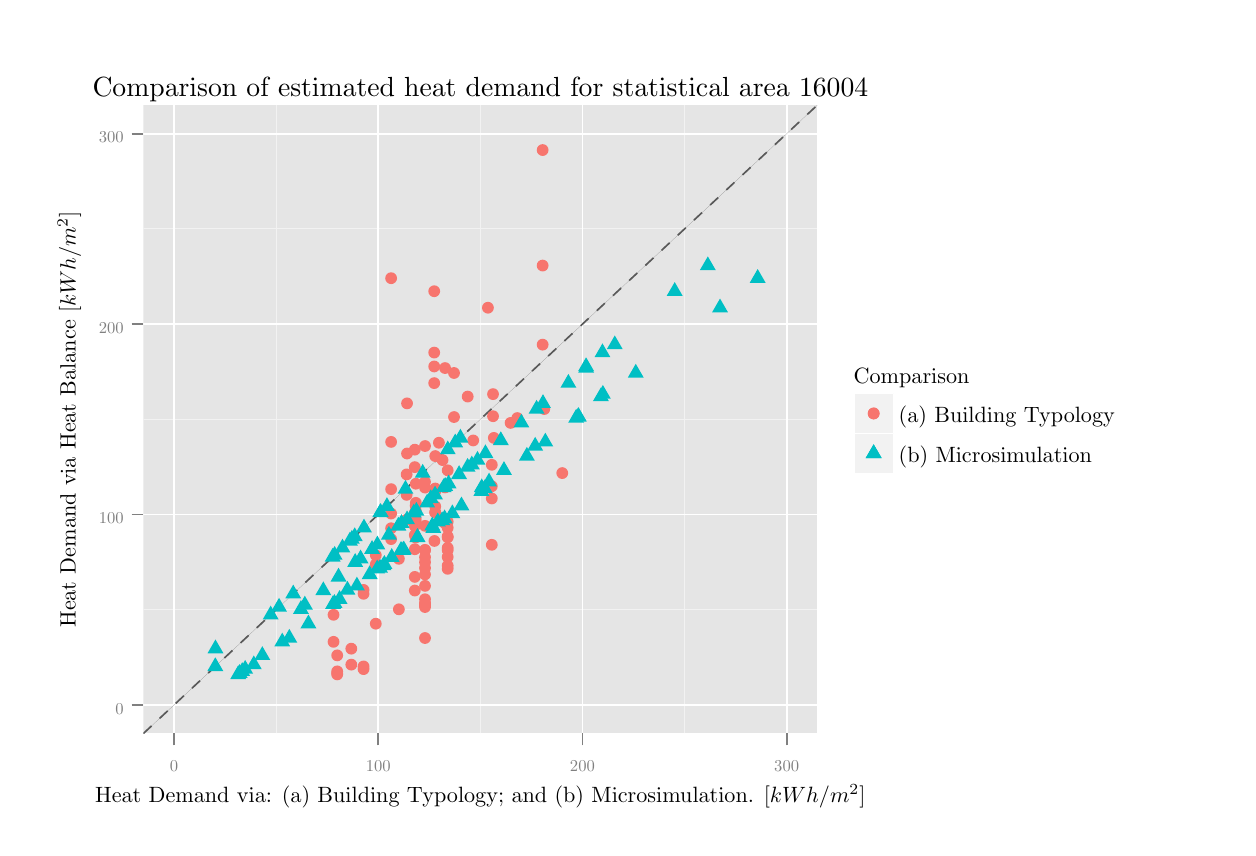
\begin{tikzpicture}[x=1pt,y=1pt]
\definecolor[named]{fillColor}{rgb}{1.00,1.00,1.00}
\path[use as bounding box,fill=fillColor,fill opacity=0.00] (0,0) rectangle (433.62,289.08);
\begin{scope}
\path[clip] (  0.00,  0.00) rectangle (433.62,289.08);
\definecolor[named]{drawColor}{rgb}{1.00,1.00,1.00}
\definecolor[named]{fillColor}{rgb}{1.00,1.00,1.00}

\path[draw=drawColor,line width= 0.6pt,line join=round,line cap=round,fill=fillColor] ( -0.00,  0.00) rectangle (433.62,289.08);
\end{scope}
\begin{scope}
\path[clip] ( 41.82, 34.03) rectangle (285.33,261.09);
\definecolor[named]{fillColor}{rgb}{0.90,0.90,0.90}

\path[fill=fillColor] ( 41.82, 34.03) rectangle (285.33,261.09);
\definecolor[named]{drawColor}{rgb}{0.95,0.95,0.95}

\path[draw=drawColor,line width= 0.3pt,line join=round] ( 41.82, 78.76) --
	(285.33, 78.76);

\path[draw=drawColor,line width= 0.3pt,line join=round] ( 41.82,147.56) --
	(285.33,147.56);

\path[draw=drawColor,line width= 0.3pt,line join=round] ( 41.82,216.37) --
	(285.33,216.37);

\path[draw=drawColor,line width= 0.3pt,line join=round] ( 89.78, 34.03) --
	( 89.78,261.09);

\path[draw=drawColor,line width= 0.3pt,line join=round] (163.58, 34.03) --
	(163.58,261.09);

\path[draw=drawColor,line width= 0.3pt,line join=round] (237.37, 34.03) --
	(237.37,261.09);
\definecolor[named]{drawColor}{rgb}{1.00,1.00,1.00}

\path[draw=drawColor,line width= 0.6pt,line join=round] ( 41.82, 44.36) --
	(285.33, 44.36);

\path[draw=drawColor,line width= 0.6pt,line join=round] ( 41.82,113.16) --
	(285.33,113.16);

\path[draw=drawColor,line width= 0.6pt,line join=round] ( 41.82,181.97) --
	(285.33,181.97);

\path[draw=drawColor,line width= 0.6pt,line join=round] ( 41.82,250.77) --
	(285.33,250.77);

\path[draw=drawColor,line width= 0.6pt,line join=round] ( 52.89, 34.03) --
	( 52.89,261.09);

\path[draw=drawColor,line width= 0.6pt,line join=round] (126.68, 34.03) --
	(126.68,261.09);

\path[draw=drawColor,line width= 0.6pt,line join=round] (200.47, 34.03) --
	(200.47,261.09);

\path[draw=drawColor,line width= 0.6pt,line join=round] (274.26, 34.03) --
	(274.26,261.09);
\definecolor[named]{drawColor}{rgb}{0.35,0.35,0.35}
\definecolor[named]{fillColor}{rgb}{0.35,0.35,0.35}

\path[draw=drawColor,line width= 0.6pt,dash pattern=on 4pt off 4pt ,line join=round,fill=fillColor] ( 41.82, 34.03) -- (285.33,261.09);
\definecolor[named]{fillColor}{rgb}{0.97,0.46,0.43}

\path[fill=fillColor] (131.33,139.40) circle (  2.13);

\path[fill=fillColor] (139.89, 90.61) circle (  2.13);

\path[fill=fillColor] (147.27,121.57) circle (  2.13);

\path[fill=fillColor] (134.13, 78.91) circle (  2.13);

\path[fill=fillColor] (186.08,244.86) circle (  2.13);

\path[fill=fillColor] (131.33,108.20) circle (  2.13);

\path[fill=fillColor] (159.00,155.78) circle (  2.13);

\path[fill=fillColor] (167.71,131.12) circle (  2.13);

\path[fill=fillColor] (147.27,116.09) circle (  2.13);

\path[fill=fillColor] (140.26,124.28) circle (  2.13);

\path[fill=fillColor] (154.06,164.30) circle (  2.13);

\path[fill=fillColor] (150.81,110.00) circle (  2.13);

\path[fill=fillColor] (143.58, 95.91) circle (  2.13);

\path[fill=fillColor] (168.15,148.68) circle (  2.13);

\path[fill=fillColor] (140.18,111.66) circle (  2.13);

\path[fill=fillColor] (136.94,127.65) circle (  2.13);

\path[fill=fillColor] (154.06,148.38) circle (  2.13);

\path[fill=fillColor] (168.45,140.84) circle (  2.13);

\path[fill=fillColor] (160.99,139.92) circle (  2.13);

\path[fill=fillColor] (143.58,100.21) circle (  2.13);

\path[fill=fillColor] (167.71,118.96) circle (  2.13);

\path[fill=fillColor] (111.85, 56.48) circle (  2.13);

\path[fill=fillColor] (166.31,187.88) circle (  2.13);

\path[fill=fillColor] (151.77,101.10) circle (  2.13);

\path[fill=fillColor] (147.27,122.55) circle (  2.13);

\path[fill=fillColor] (121.37, 85.91) circle (  2.13);

\path[fill=fillColor] (151.77,110.57) circle (  2.13);

\path[fill=fillColor] (143.58,122.88) circle (  2.13);

\path[fill=fillColor] (151.77,108.35) circle (  2.13);

\path[fill=fillColor] (136.94,111.31) circle (  2.13);

\path[fill=fillColor] (139.89,109.03) circle (  2.13);

\path[fill=fillColor] (167.71,102.21) circle (  2.13);

\path[fill=fillColor] (151.77,105.23) circle (  2.13);

\path[fill=fillColor] (174.50,146.26) circle (  2.13);

\path[fill=fillColor] (125.79, 98.47) circle (  2.13);

\path[fill=fillColor] (143.58, 81.10) circle (  2.13);

\path[fill=fillColor] (111.85, 55.38) circle (  2.13);

\path[fill=fillColor] (143.58, 82.54) circle (  2.13);

\path[fill=fillColor] (140.18,110.98) circle (  2.13);

\path[fill=fillColor] (150.81,122.94) circle (  2.13);

\path[fill=fillColor] (131.33,113.51) circle (  2.13);

\path[fill=fillColor] (139.89,113.74) circle (  2.13);

\path[fill=fillColor] (143.58, 80.49) circle (  2.13);

\path[fill=fillColor] (110.52, 76.92) circle (  2.13);

\path[fill=fillColor] (131.33,122.33) circle (  2.13);

\path[fill=fillColor] (151.77,129.13) circle (  2.13);

\path[fill=fillColor] (125.79, 95.18) circle (  2.13);

\path[fill=fillColor] (143.58, 80.73) circle (  2.13);

\path[fill=fillColor] (186.08,203.12) circle (  2.13);

\path[fill=fillColor] (146.90,193.84) circle (  2.13);

\path[fill=fillColor] (176.93,148.01) circle (  2.13);

\path[fill=fillColor] (121.37, 57.30) circle (  2.13);

\path[fill=fillColor] (143.58,124.96) circle (  2.13);

\path[fill=fillColor] (134.13, 97.15) circle (  2.13);

\path[fill=fillColor] (143.58,100.39) circle (  2.13);

\path[fill=fillColor] (147.27,134.27) circle (  2.13);

\path[fill=fillColor] (139.89, 85.69) circle (  2.13);

\path[fill=fillColor] (151.77, 94.68) circle (  2.13);

\path[fill=fillColor] (148.60,139.09) circle (  2.13);

\path[fill=fillColor] (140.18,104.84) circle (  2.13);

\path[fill=fillColor] (139.89,136.59) circle (  2.13);

\path[fill=fillColor] (111.85, 55.82) circle (  2.13);

\path[fill=fillColor] (116.94, 64.68) circle (  2.13);

\path[fill=fillColor] (186.67,151.27) circle (  2.13);

\path[fill=fillColor] (167.71,123.37) circle (  2.13);

\path[fill=fillColor] (147.27,113.83) circle (  2.13);

\path[fill=fillColor] (143.58, 91.51) circle (  2.13);

\path[fill=fillColor] (131.33,198.55) circle (  2.13);

\path[fill=fillColor] (193.17,128.13) circle (  2.13);

\path[fill=fillColor] (121.37, 84.51) circle (  2.13);

\path[fill=fillColor] (140.26,114.40) circle (  2.13);

\path[fill=fillColor] (139.89,100.61) circle (  2.13);

\path[fill=fillColor] (125.79, 73.70) circle (  2.13);

\path[fill=fillColor] (111.85, 62.26) circle (  2.13);

\path[fill=fillColor] (136.94,120.26) circle (  2.13);

\path[fill=fillColor] (150.81,166.08) circle (  2.13);

\path[fill=fillColor] (140.18,116.34) circle (  2.13);

\path[fill=fillColor] (131.33,104.27) circle (  2.13);

\path[fill=fillColor] (143.58, 93.81) circle (  2.13);

\path[fill=fillColor] (139.89,105.76) circle (  2.13);

\path[fill=fillColor] (139.89,130.28) circle (  2.13);

\path[fill=fillColor] (149.92,132.83) circle (  2.13);

\path[fill=fillColor] (110.52, 67.15) circle (  2.13);

\path[fill=fillColor] (151.77, 93.54) circle (  2.13);

\path[fill=fillColor] (137.08,135.20) circle (  2.13);

\path[fill=fillColor] (121.37, 58.26) circle (  2.13);

\path[fill=fillColor] (137.08,153.32) circle (  2.13);

\path[fill=fillColor] (116.94, 58.91) circle (  2.13);

\path[fill=fillColor] (143.58,137.90) circle (  2.13);

\path[fill=fillColor] (143.58, 87.37) circle (  2.13);

\path[fill=fillColor] (146.90,171.67) circle (  2.13);

\path[fill=fillColor] (168.15,156.66) circle (  2.13);

\path[fill=fillColor] (186.08,174.54) circle (  2.13);

\path[fill=fillColor] (143.58, 68.53) circle (  2.13);

\path[fill=fillColor] (151.77,104.90) circle (  2.13);

\path[fill=fillColor] (140.26,117.37) circle (  2.13);

\path[fill=fillColor] (147.27,113.98) circle (  2.13);

\path[fill=fillColor] (146.97,103.60) circle (  2.13);

\path[fill=fillColor] (143.58,109.06) circle (  2.13);

\path[fill=fillColor] (146.90,160.64) circle (  2.13);

\path[fill=fillColor] (151.77,100.26) circle (  2.13);

\path[fill=fillColor] (151.77, 97.81) circle (  2.13);

\path[fill=fillColor] (143.58, 79.73) circle (  2.13);

\path[fill=fillColor] (143.58, 97.71) circle (  2.13);

\path[fill=fillColor] (146.90,166.65) circle (  2.13);
\definecolor[named]{fillColor}{rgb}{0.00,0.75,0.77}

\path[fill=fillColor] (187.05,142.72) --
	(189.92,137.74) --
	(184.17,137.74) --
	cycle;

\path[fill=fillColor] (112.33, 93.93) --
	(115.20, 88.95) --
	(109.46, 88.95) --
	cycle;

\path[fill=fillColor] (163.94,124.88) --
	(166.82,119.91) --
	(161.07,119.91) --
	cycle;

\path[fill=fillColor] ( 98.74, 82.23) --
	(101.61, 77.25) --
	( 95.87, 77.25) --
	cycle;

\path[fill=fillColor] (146.56,111.52) --
	(149.44,106.54) --
	(143.69,106.54) --
	cycle;

\path[fill=fillColor] (207.14,159.10) --
	(210.01,154.12) --
	(204.26,154.12) --
	cycle;

\path[fill=fillColor] (160.49,134.44) --
	(163.37,129.46) --
	(157.62,129.46) --
	cycle;

\path[fill=fillColor] (129.82,119.41) --
	(132.70,114.43) --
	(126.95,114.43) --
	cycle;

\path[fill=fillColor] (152.09,127.60) --
	(154.97,122.62) --
	(149.22,122.62) --
	cycle;

\path[fill=fillColor] (219.73,167.62) --
	(222.60,162.64) --
	(216.86,162.64) --
	cycle;

\path[fill=fillColor] (135.08,113.32) --
	(137.96,108.34) --
	(132.21,108.34) --
	cycle;

\path[fill=fillColor] (118.34, 99.23) --
	(121.22, 94.25) --
	(115.47, 94.25) --
	cycle;

\path[fill=fillColor] (198.97,151.99) --
	(201.85,147.02) --
	(196.10,147.02) --
	cycle;

\path[fill=fillColor] (150.66,114.98) --
	(153.53,110.00) --
	(147.78,110.00) --
	cycle;

\path[fill=fillColor] (155.89,130.97) --
	(158.76,125.99) --
	(153.01,125.99) --
	cycle;

\path[fill=fillColor] (199.13,151.70) --
	(202.01,146.72) --
	(196.26,146.72) --
	cycle;

\path[fill=fillColor] (156.36,144.16) --
	(159.24,139.18) --
	(153.49,139.18) --
	cycle;

\path[fill=fillColor] (170.96,143.24) --
	(173.84,138.26) --
	(168.09,138.26) --
	cycle;

\path[fill=fillColor] (135.69,103.53) --
	(138.56, 98.55) --
	(132.81, 98.55) --
	cycle;

\path[fill=fillColor] (145.66,122.28) --
	(148.54,117.30) --
	(142.79,117.30) --
	cycle;

\path[fill=fillColor] ( 77.52, 59.80) --
	( 80.39, 54.82) --
	( 74.65, 54.82) --
	cycle;

\path[fill=fillColor] (250.18,191.20) --
	(253.05,186.22) --
	(247.31,186.22) --
	cycle;

\path[fill=fillColor] (113.75,104.42) --
	(116.62, 99.44) --
	(110.87, 99.44) --
	cycle;

\path[fill=fillColor] (165.19,125.87) --
	(168.06,120.89) --
	(162.32,120.89) --
	cycle;

\path[fill=fillColor] (115.54, 89.22) --
	(118.41, 84.25) --
	(112.66, 84.25) --
	cycle;

\path[fill=fillColor] (148.20,113.89) --
	(151.08,108.91) --
	(145.33,108.91) --
	cycle;

\path[fill=fillColor] (164.07,126.20) --
	(166.95,121.22) --
	(161.20,121.22) --
	cycle;

\path[fill=fillColor] (121.52,111.67) --
	(124.40,106.69) --
	(118.65,106.69) --
	cycle;

\path[fill=fillColor] (137.09,114.63) --
	(139.96,109.65) --
	(134.22,109.65) --
	cycle;

\path[fill=fillColor] (133.96,112.35) --
	(136.84,107.37) --
	(131.09,107.37) --
	cycle;

\path[fill=fillColor] (126.37,105.53) --
	(129.24,100.55) --
	(123.50,100.55) --
	cycle;

\path[fill=fillColor] (118.18,108.55) --
	(121.05,103.57) --
	(115.30,103.57) --
	cycle;

\path[fill=fillColor] (178.41,149.58) --
	(181.28,144.61) --
	(175.53,144.61) --
	cycle;

\path[fill=fillColor] (110.93,101.79) --
	(113.80, 96.82) --
	(108.06, 96.82) --
	cycle;

\path[fill=fillColor] (110.88, 84.41) --
	(113.75, 79.44) --
	(108.00, 79.44) --
	cycle;

\path[fill=fillColor] ( 76.08, 58.70) --
	( 78.95, 53.72) --
	( 73.21, 53.72) --
	cycle;

\path[fill=fillColor] (112.70, 85.86) --
	(115.57, 80.88) --
	(109.83, 80.88) --
	cycle;

\path[fill=fillColor] (149.77,114.30) --
	(152.65,109.32) --
	(146.90,109.32) --
	cycle;

\path[fill=fillColor] (150.32,126.26) --
	(153.19,121.28) --
	(147.44,121.28) --
	cycle;

\path[fill=fillColor] (153.46,116.83) --
	(156.33,111.85) --
	(150.59,111.85) --
	cycle;

\path[fill=fillColor] (139.52,117.05) --
	(142.40,112.08) --
	(136.65,112.08) --
	cycle;

\path[fill=fillColor] (100.15, 83.81) --
	(103.03, 78.83) --
	( 97.28, 78.83) --
	cycle;

\path[fill=fillColor] ( 87.81, 80.24) --
	( 90.68, 75.26) --
	( 84.94, 75.26) --
	cycle;

\path[fill=fillColor] (136.51,125.65) --
	(139.39,120.67) --
	(133.64,120.67) --
	cycle;

\path[fill=fillColor] (172.11,132.45) --
	(174.99,127.47) --
	(169.24,127.47) --
	cycle;

\path[fill=fillColor] (128.91, 98.50) --
	(131.79, 93.52) --
	(126.04, 93.52) --
	cycle;

\path[fill=fillColor] (110.35, 84.05) --
	(113.22, 79.07) --
	(107.48, 79.07) --
	cycle;

\path[fill=fillColor] (245.77,206.43) --
	(248.64,201.46) --
	(242.89,201.46) --
	cycle;

\path[fill=fillColor] (233.80,197.16) --
	(236.67,192.18) --
	(230.92,192.18) --
	cycle;

\path[fill=fillColor] (198.19,151.33) --
	(201.07,146.35) --
	(195.32,146.35) --
	cycle;

\path[fill=fillColor] ( 78.59, 60.61) --
	( 81.47, 55.64) --
	( 75.72, 55.64) --
	cycle;

\path[fill=fillColor] (166.72,128.28) --
	(169.59,123.30) --
	(163.85,123.30) --
	cycle;

\path[fill=fillColor] (120.29,100.47) --
	(123.17, 95.50) --
	(117.42, 95.50) --
	cycle;

\path[fill=fillColor] (135.92,103.71) --
	(138.80, 98.73) --
	(133.05, 98.73) --
	cycle;

\path[fill=fillColor] (180.38,137.59) --
	(183.26,132.61) --
	(177.51,132.61) --
	cycle;

\path[fill=fillColor] (106.83, 89.00) --
	(109.71, 84.03) --
	(103.96, 84.03) --
	cycle;

\path[fill=fillColor] (128.56, 98.00) --
	(131.44, 93.02) --
	(125.69, 93.02) --
	cycle;

\path[fill=fillColor] (154.49,142.41) --
	(157.36,137.43) --
	(151.62,137.43) --
	cycle;

\path[fill=fillColor] (140.84,108.16) --
	(143.71,103.18) --
	(137.97,103.18) --
	cycle;

\path[fill=fillColor] (151.81,139.91) --
	(154.68,134.94) --
	(148.94,134.94) --
	cycle;

\path[fill=fillColor] ( 76.60, 59.13) --
	( 79.47, 54.16) --
	( 73.73, 54.16) --
	cycle;

\path[fill=fillColor] ( 67.86, 68.00) --
	( 70.74, 63.02) --
	( 64.99, 63.02) --
	cycle;

\path[fill=fillColor] (183.89,154.59) --
	(186.76,149.61) --
	(181.01,149.61) --
	cycle;

\path[fill=fillColor] (150.86,126.69) --
	(153.73,121.71) --
	(147.98,121.71) --
	cycle;

\path[fill=fillColor] (127.39,117.14) --
	(130.27,112.17) --
	(124.52,112.17) --
	cycle;

\path[fill=fillColor] (123.60, 94.83) --
	(126.47, 89.85) --
	(120.72, 89.85) --
	cycle;

\path[fill=fillColor] (263.78,201.87) --
	(266.66,196.89) --
	(260.91,196.89) --
	cycle;

\path[fill=fillColor] (142.74,131.45) --
	(145.61,126.47) --
	(139.86,126.47) --
	cycle;

\path[fill=fillColor] ( 95.96, 87.83) --
	( 98.83, 82.85) --
	( 93.08, 82.85) --
	cycle;

\path[fill=fillColor] (140.47,117.72) --
	(143.35,112.74) --
	(137.60,112.74) --
	cycle;

\path[fill=fillColor] (124.44,103.93) --
	(127.32, 98.95) --
	(121.57, 98.95) --
	cycle;

\path[fill=fillColor] (101.45, 77.02) --
	(104.32, 72.04) --
	( 98.57, 72.04) --
	cycle;

\path[fill=fillColor] ( 84.79, 65.58) --
	( 87.66, 60.60) --
	( 81.92, 60.60) --
	cycle;

\path[fill=fillColor] (147.20,123.58) --
	(150.07,118.60) --
	(144.32,118.60) --
	cycle;

\path[fill=fillColor] (201.81,169.40) --
	(204.68,164.42) --
	(198.93,164.42) --
	cycle;

\path[fill=fillColor] (156.75,119.65) --
	(159.62,114.68) --
	(153.87,114.68) --
	cycle;

\path[fill=fillColor] (117.14,107.59) --
	(120.02,102.61) --
	(114.27,102.61) --
	cycle;

\path[fill=fillColor] (127.33, 97.13) --
	(130.20, 92.15) --
	(124.45, 92.15) --
	cycle;

\path[fill=fillColor] (130.53,109.08) --
	(133.40,104.10) --
	(127.65,104.10) --
	cycle;

\path[fill=fillColor] (158.97,133.60) --
	(161.84,128.62) --
	(156.10,128.62) --
	cycle;

\path[fill=fillColor] (162.54,136.14) --
	(165.41,131.17) --
	(159.67,131.17) --
	cycle;

\path[fill=fillColor] ( 91.99, 70.47) --
	( 94.87, 65.49) --
	( 89.12, 65.49) --
	cycle;

\path[fill=fillColor] (126.29, 96.86) --
	(129.17, 91.88) --
	(123.42, 91.88) --
	cycle;

\path[fill=fillColor] (165.41,138.51) --
	(168.29,133.54) --
	(162.54,133.54) --
	cycle;

\path[fill=fillColor] ( 67.80, 61.58) --
	( 70.68, 56.60) --
	( 64.93, 56.60) --
	cycle;

\path[fill=fillColor] (186.21,156.64) --
	(189.08,151.66) --
	(183.34,151.66) --
	cycle;

\path[fill=fillColor] ( 81.71, 62.23) --
	( 84.59, 57.25) --
	( 78.84, 57.25) --
	cycle;

\path[fill=fillColor] (183.39,141.22) --
	(186.26,136.24) --
	(180.51,136.24) --
	cycle;

\path[fill=fillColor] (118.97, 90.69) --
	(121.85, 85.71) --
	(116.10, 85.71) --
	cycle;

\path[fill=fillColor] (207.69,174.99) --
	(210.56,170.01) --
	(204.82,170.01) --
	cycle;

\path[fill=fillColor] (207.85,159.98) --
	(210.72,155.00) --
	(204.97,155.00) --
	cycle;

\path[fill=fillColor] (212.15,177.86) --
	(215.02,172.89) --
	(209.27,172.89) --
	cycle;

\path[fill=fillColor] ( 94.55, 71.84) --
	( 97.42, 66.87) --
	( 91.68, 66.87) --
	cycle;

\path[fill=fillColor] (140.86,108.22) --
	(143.73,103.24) --
	(137.98,103.24) --
	cycle;

\path[fill=fillColor] (144.35,120.68) --
	(147.23,115.71) --
	(141.48,115.71) --
	cycle;

\path[fill=fillColor] (127.55,117.29) --
	(130.43,112.32) --
	(124.68,112.32) --
	cycle;

\path[fill=fillColor] (116.42,106.92) --
	(119.30,101.94) --
	(113.55,101.94) --
	cycle;

\path[fill=fillColor] (146.21,112.38) --
	(149.09,107.40) --
	(143.34,107.40) --
	cycle;

\path[fill=fillColor] (195.39,163.96) --
	(198.27,158.98) --
	(192.52,158.98) --
	cycle;

\path[fill=fillColor] (134.92,103.58) --
	(137.79, 98.60) --
	(132.05, 98.60) --
	cycle;

\path[fill=fillColor] (110.21,101.13) --
	(113.09, 96.15) --
	(107.34, 96.15) --
	cycle;

\path[fill=fillColor] ( 90.83, 83.05) --
	( 93.70, 78.08) --
	( 87.96, 78.08) --
	cycle;

\path[fill=fillColor] (131.55,101.03) --
	(134.42, 96.05) --
	(128.68, 96.05) --
	cycle;

\path[fill=fillColor] (201.78,169.97) --
	(204.65,164.99) --
	(198.91,164.99) --
	cycle;
\end{scope}
\begin{scope}
\path[clip] (  0.00,  0.00) rectangle (433.62,289.08);
\definecolor[named]{drawColor}{rgb}{0.50,0.50,0.50}

\node[text=drawColor,anchor=base east,inner sep=0pt, outer sep=0pt, scale= 0.6]
at ( 34.71, 41.05) {0};

\node[text=drawColor,anchor=base east,inner sep=0pt, outer sep=0pt, scale=  0.6] at ( 34.71,109.86) {100};

\node[text=drawColor,anchor=base east,inner sep=0pt, outer sep=0pt, scale=  0.6] at ( 34.71,178.66) {200};

\node[text=drawColor,anchor=base east,inner sep=0pt, outer sep=0pt, scale=  0.6] at ( 34.71,247.47) {300};
\end{scope}
\begin{scope}
\path[clip] (  0.00,  0.00) rectangle (433.62,289.08);
\definecolor[named]{drawColor}{rgb}{0.50,0.50,0.50}

\path[draw=drawColor,line width= 0.6pt,line join=round] ( 37.55, 44.36) --
	( 41.82, 44.36);

\path[draw=drawColor,line width= 0.6pt,line join=round] ( 37.55,113.16) --
	( 41.82,113.16);

\path[draw=drawColor,line width= 0.6pt,line join=round] ( 37.55,181.97) --
	( 41.82,181.97);

\path[draw=drawColor,line width= 0.6pt,line join=round] ( 37.55,250.77) --
	( 41.82,250.77);
\end{scope}
\begin{scope}
\path[clip] (  0.00,  0.00) rectangle (433.62,289.08);
\definecolor[named]{drawColor}{rgb}{0.50,0.50,0.50}

\path[draw=drawColor,line width= 0.6pt,line join=round] ( 52.89, 29.77) --
	( 52.89, 34.03);

\path[draw=drawColor,line width= 0.6pt,line join=round] (126.68, 29.77) --
	(126.68, 34.03);

\path[draw=drawColor,line width= 0.6pt,line join=round] (200.47, 29.77) --
	(200.47, 34.03);

\path[draw=drawColor,line width= 0.6pt,line join=round] (274.26, 29.77) --
	(274.26, 34.03);
\end{scope}
\begin{scope}
\path[clip] (  0.00,  0.00) rectangle (433.62,289.08);
\definecolor[named]{drawColor}{rgb}{0.50,0.50,0.50}

\node[text=drawColor,anchor=base,inner sep=0pt, outer sep=0pt, scale= 0.6] at (
52.89, 20.31) {0};

\node[text=drawColor,anchor=base,inner sep=0pt, outer sep=0pt, scale=  0.6] at (126.68, 20.31) {100};

\node[text=drawColor,anchor=base,inner sep=0pt, outer sep=0pt, scale=  0.6] at (200.47, 20.31) {200};

\node[text=drawColor,anchor=base,inner sep=0pt, outer sep=0pt, scale=  0.6] at (274.26, 20.31) {300};
\end{scope}
\begin{scope}
\path[clip] (  0.00,  0.00) rectangle (433.62,289.08);
\definecolor[named]{drawColor}{rgb}{0.00,0.00,0.00}

\node[text=drawColor,anchor=base,inner sep=0pt, outer sep=0pt, scale= 0.8] at
(163.58,  9.03) {Heat Demand via: (a) Building Typology; and (b) Microsimulation. $[kWh/m^2]$};
\end{scope}
\begin{scope}
\path[clip] (  0.00,  0.00) rectangle (433.62,289.08);
\definecolor[named]{drawColor}{rgb}{0.00,0.00,0.00}

\node[text=drawColor,rotate= 90.00,anchor=base,inner sep=0pt, outer sep=0pt,
scale= 0.8] at ( 17.30,147.56) {Heat Demand via Heat Balance $[kWh/m^2]$};
\end{scope}
\begin{scope}
\path[clip] (  0.00,  0.00) rectangle (433.62,289.08);
\definecolor[named]{fillColor}{rgb}{1.00,1.00,1.00}

\path[fill=fillColor] (294.20,123.72) rectangle (412.71,171.41);
\end{scope}
\begin{scope}
\path[clip] (  0.00,  0.00) rectangle (433.62,289.08);
\definecolor[named]{drawColor}{rgb}{0.00,0.00,0.00}

\node[text=drawColor,anchor=base west,inner sep=0pt, outer sep=0pt, scale= 
0.8] at (298.47,160.51) {Comparison};
\end{scope}
\begin{scope}
\path[clip] (  0.00,  0.00) rectangle (433.62,289.08);
\definecolor[named]{drawColor}{rgb}{1.00,1.00,1.00}
\definecolor[named]{fillColor}{rgb}{0.95,0.95,0.95}

\path[draw=drawColor,line width= 0.6pt,line join=round,line
cap=round,fill=fillColor] (298.47,142.45) rectangle (312.92,156.90);
\end{scope}
\begin{scope}
\path[clip] (  0.00,  0.00) rectangle (433.62,289.08);
\definecolor[named]{fillColor}{rgb}{0.97,0.46,0.43}

\path[fill=fillColor] (305.69,149.67) circle (  2.13);
\end{scope}
\begin{scope}
\path[clip] (  0.00,  0.00) rectangle (433.62,289.08);
\definecolor[named]{fillColor}{rgb}{0.97,0.46,0.43}

\path[fill=fillColor] (305.69,149.67) circle (  2.13);
\end{scope}
\begin{scope}
\path[clip] (  0.00,  0.00) rectangle (433.62,289.08);
\definecolor[named]{drawColor}{rgb}{1.00,1.00,1.00}
\definecolor[named]{fillColor}{rgb}{0.95,0.95,0.95}

\path[draw=drawColor,line width= 0.6pt,line join=round,line
cap=round,fill=fillColor] (298.47,127.99) rectangle (312.92,142.45);
\end{scope}
\begin{scope}
\path[clip] (  0.00,  0.00) rectangle (433.62,289.08);
\definecolor[named]{fillColor}{rgb}{0.00,0.75,0.77}

\path[fill=fillColor] (305.69,138.54) --
	(308.57,133.56) --
	(302.82,133.56) --
	cycle;
\end{scope}
\begin{scope}
\path[clip] (  0.00,  0.00) rectangle (433.62,289.08);
\definecolor[named]{fillColor}{rgb}{0.00,0.75,0.77}

\path[fill=fillColor] (305.69,138.54) --
	(308.57,133.56) --
	(302.82,133.56) --
	cycle;
\end{scope}
\begin{scope}
\path[clip] (  0.00,  0.00) rectangle (433.62,289.08);
\definecolor[named]{drawColor}{rgb}{0.00,0.00,0.00}

\node[text=drawColor,anchor=base west,inner sep=0pt, outer sep=0pt, scale= 
0.8] at (314.73,146.37) {(a) Building Typology};
\end{scope}
\begin{scope}
\path[clip] (  0.00,  0.00) rectangle (433.62,289.08);
\definecolor[named]{drawColor}{rgb}{0.00,0.00,0.00}

\node[text=drawColor,anchor=base west,inner sep=0pt, outer sep=0pt, scale= 
0.8] at (314.73,131.91) {(b) Microsimulation};
\end{scope}
\begin{scope}
\path[clip] (  0.00,  0.00) rectangle (433.62,289.08);
\definecolor[named]{drawColor}{rgb}{0.00,0.00,0.00}

\node[text=drawColor,anchor=base,inner sep=0pt, outer sep=0pt, scale= 1] at
(163.58,264.11) {Comparison of estimated heat demand for statistical area 16004};
\end{scope}
\end{tikzpicture}
